
\pagebreak

\subsection{Milky Way Scan}

\subsubsection{Observation time}
From our observation spot in Bern, we had to plan the observation time to get the best possible overview of the Milky Way with a wide range in the galactic longitude. In October, when we did this measurments, the maximum elevation of the galactic center is around 13° (in south) at 18:30 MESZ. However, limitations in the field of view of the SRT had to be considered to choose the best observation time:

\begin{itemize}
    \item At 18:30 MESZ, the galactic center ($l_g=\SI{0}{\degree}$) could be included in the scan but at galactic longitudes of $l_g>\SI{120}{\degree}$, the SRT run in the lower azimuth limit from EXWI building at around 40° (north east).
    \item At later times, the galactic center is already descending and but the higher galactic longitudes are moving inside visible area of the SRT.
    \item At 22:00 MESZ, the galactic center is at the horizon and no more visible but the galactic plane is almost perpendicular to the horizontal plane and it is in the visible area of the SRT up to galactic longitude $l_g=\SI{180}{\degree}$. Only limitation is the main building of the University Bern, that covers the view partially. We decided to do the scan at this time. 
\end{itemize}
    
The scan path is illustrated in figure \ref{fig:mw_scan_stellarium}. We chose the scan path start at galactic longitude of 10° and end at 170° to avoid lower elevations than 10° as the noise level of the ground thermal radiation is dominating there.


\begin{figure}[H]
    \centering
    \includegraphics[width=12cm]{assets/stellariumView_edit.png}
    \caption{View of the Milky Way scan in Stellarium [XXX] with SRT field of view limitations (blue).}
    \label{fig:mw_scan_stellarium}
\end{figure}

\subsubsection{Measurement}
It was hard to find out, how to correctly set up the LAb View tool for a Milky Way scan, as the angular range input fields belong to azimuthal coordinates rather than galactic. Finally we found, that the tool uses wrong (mirrored) galactic coordinates (correct longitude is $l_g=\SI{360}{\degree}-l_{srt}$ to enter in the azimuth fields. We chose a step size of $\Delta l_g=\SI{0.25}{\degree}$ with 1000 ms integration time what resulted in a measurement time of 28 min to scan from 10° to 170° in galactic coordinates. Figure \ref{fig:mw_scan_polar} shows the scan path in a polar diagram:

\begin{figure}[H]
    \centering
    \includegraphics[width=10cm]{assets/mw_scan_polar.png}
    \caption{Polar plot of the Milky Way scan}
    \label{fig:mw_scan_polar}
\end{figure}

Figure \ref{fig:mw_spectrum_plot} shows the received power spectrum of the Milky Way scan. Frequencies above the carrier frequency $f_c$ are BLABLA............
some interesting regions are marked in red and will be discussed later.


\begin{figure}[H]
    \centering
    \includegraphics[width=\textwidth]{assets/spectrum_plot_edit.png}
    \caption{Received spectral power density vs. galactic longitude @ at zero latitude (galactic plane)}
    \label{fig:mw_spectrum_plot}
\end{figure}

We can point out following features in the spectrum plot:

\begin{itemize}
    \item We see a clear trend of maximum power 
    \item Bla
    \item Blue shift offset in tangential direction. 
    In tangential direction 
\end{itemize}

\subsubsection{Qualitative analysis of the hot spots}


\begin{figure}[H]
    \centering
    \includegraphics[width=\textwidth]{assets/MW_ROI_spots.png}
    \caption{Bla}
    \label{fig:mw_roi_spots}
\end{figure}


